
Uma \gls{bn} provê uma representação compacta de distribuições de probabilidades grandes demais para lidar usando especificações tradicionais e provê um método sistemático e localizado para incorporar informação probabilística sobre uma dada situação.

Uma BN é um \gls{dag} que representa uma função de distribuição de probabilidades conjunta de variáveis que modelam certo domínio de conhecimento. Ela é constituída de uma \gls{dag}, de variáveis aleatórias (também chamadas de nós da rede), arcos direcionados da variável pai para a variável filha e uma \gls{cpt} associada a cada variável.
\begin{figure}[H]
	\centering
	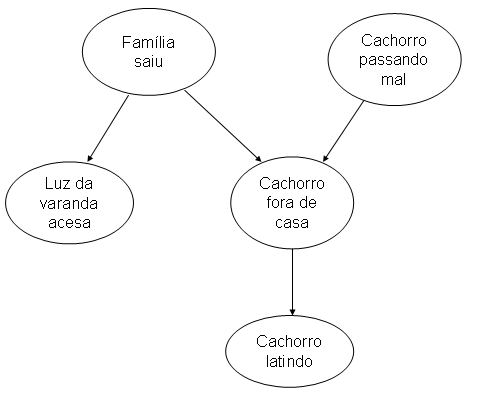
\includegraphics[width = 300px]{figuras/BN1}
	\caption[Exemplo family-out]{Exemplo family-out}
	\label{fig:familyBN}
\end{figure}

Nesse exemplo, suponhamos que se queira determinar se a família está em casa ou se ela saiu. Pelo grafo, podemos perceber que o fato de a luz da varanda estar acesa e de o cachorro estar fora de casa são indícios de que a família tenha saído. 

Nas últimas décadas, redes Bayesianas se tornaram representações populares para codificar conhecimento incerto para sistemas especialistas \cite{heck95}. Mais recentemente, pesquisadores desenvolveram métodos de aprendizagem de redes Bayesianas a partir de dados. As técnicas desenvolvidas são relativamente novas e ainda em evolução, mas eles têm se mostrado muito eficientes para alguns problemas de análise de dados.

Existem diversos representações possíveis para analise de dados, entre elas, decision tres, e redes neurais artificiais; e outras tantas como estimação de densidade, classificação, regressão e clusterings. Portanto o que métodos de \glspl{bn} têm a oferecer? Segundo Heckerman \cite{heck95} podemos oferecer pelo menos quatro respostas, sendo elas:

\begin{enumerate}
	\item \glspl{bn} lidam com um conjunto incompleto de dados de maneira natural.
	
	\item \glspl{bn} permitem aprender sobre as relações causais. Aprender sobre tais relações são importantes por pelo menos duas razões: O processo é útil quando se está tentando entender sobre um dado problema de domínio, como por exemplo, durante uma análise de dados exploratória.  E mais, conhecimento de relações causais nos permitem fazer predições na presença de intervenções. Por exemplo, um analista de mercado pode querer saber se é lucrativo aumentar o investimento em determinada propaganda para aumentar as vendas de seu produto. Para responder esta pergunta o analista pode determinar se esta propaganda é a causa para o aumento de suas vendas, e em caso afirmativo, quanto. O uso de \glspl{bn} nos ajuda a responder tal pergunta até mesmo quando não há experimentos nos efeitos de tal propaganda.
	
	\item \glspl{bn} em conjunto com técnicas estatísticas bayesianas facilitam a combinação de conhecimento de domínio e dados. Qualquer um que tenha feito uma análise do mundo real sabe a importância de conhecimento prévio ou de domínio, em especial quando os dados são poucos ou caros. Pelo fato de alguns sistemas comerciais (i.e., sistemas especialistas) podem ser construídos a partir de conhecimentos prévios. \cglspl{bn} possuem uma semântica causal que permitem conhecimentos prévios serem representados de uma forma muito simples e natural. Além disto, \glspl{bn} encapsulam tais relações causais com suas probabilidades. Consequentemente, conhecimento prévio e dados podem ser combinados com técnicas bem estudadas da estatística Bayesiana.
	
	\item Métodos Bayesianos em conjunto com \glspl{bn} e outros tipos de modelos oferecem uma forma eficiente para evitar over fitting dos dados. Não há necessidade de excluir parte dos dados do treinamento do aprendizado da rede. Usando técnicas Bayesianas, modelos podem ser "suavizados" de tal forma que todo dado disponível pode ser usado para o treinamento.
	
\end{enumerate}

Neste capítulo oferecemos a definição formal de \gls{bn} e introduzimos a propriedade de d-separation. Segundo J. Pearl \cite{pearl88}, é esta propriedade que permite \glspl{bn} serem um formalismo tão robusto para lidar com incerteza, pois é o que nos permite ignorar informação que não é importante. "Permissão para ignorar é o que dá combustível para sistemas semânticos" completa ele.

\section{Distribuição de Probabilidade Disjunta da Rede Bayesiana}
Considere a \gls{bn} contendo $n$ nós, $X_1$ até $X_n$, tomados nesta ordem. Uma instanciação da distribuição disjunta de probabilidade é representada por $P(X_1 = x_1, X_2 = x_2, ... , X_n = x_n)$, ou de forma compacta $P(x_1, x_2, ..., x_n)$. A \textbf{regra da cadeia} nos permite fatorar probabilidades disjuntas como:
\begin{equation}
	P(x_1, x_2, ..., x_n) = P(x_1)P(x_2|x_1)...P(x_n|x_1,..,x_{n-1})\\
	= \prod_{i}^{}P(x_i|x_1,...,x_{i-1})
\end{equation}
No entanto, a estrutura de uma \gls{bn} implica que o valor de um nó em particular é condicionado apenas aos valores dos nós pais, o que reduz a equação acima à:
\begin{equation}\label{eq:pearl}
P(x_1, x_2, ..., x_n) = \prod_i P(x_i|pa_i)
\end{equation}
Onde $pa_i$ são os nós pais de $x_i$

\section{D-separation}
Segundo Cheng\cite{cheng02} Uma rede bayesiana pode ser vista como um sistema de rede de canais de informação, onde cada não é uma válvula que está aberta ou fechada e as válvulas são conectadas por canais de informação ruidosos (arestas). O fluxo de informação pode passar por um válvula aberta, mas não por uma válvula fechada. Quando todas as válvulas sobre um caminho entre dois não estão abertas, diz-se que este caminho é aberto. Se qualquer válvula no caminho está fechada, diz-se que o caminho é fechado.

Formalmente um caminho c é dito ser d-separado (ou bloqueado) por um conjunto de nós \textbf{Z} se e somente se:
\begin{itemize}
	\item c contem uma cadeia i $\rightarrow$ m $\rightarrow$ j ou uma divergência i $\leftarrow$ m $\rightarrow$ j tal que o nó do meio m está em \textbf{Z};
	\item c contem uma convergência (ou colisor) i $\rightarrow$ m $\leftarrow$ j tal que o nó do meio não está em $\textbf{Z}$ e nenhum descendente de m está em $\textbf{Z}$
\end{itemize}

O conjunto \textbf{Z} d-separa \textbf{X} de \textbf{Y} se e somente se, \textbf{Z} bloqueia todos os caminhos de nós em \textbf{X} para nós em \textbf{Y}.

Se um caminho satisfaz a condição acima, diz-se que ele é bloqueado; caso contrário ele é ativado por \textbf{Z}. Na figura \ref{fig:d-sep} $X$ = {2} e $Y$ = {3} são d-separados por Z = {1}; o caminho 2 $\leftarrow$ 1 $\rightarrow$ 3 é bloqueado por 1 $\in$ \textbf{Z}.
\begin{figure}[H]
	\centering
	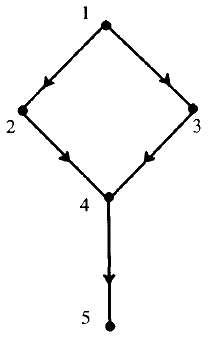
\includegraphics{figuras/d-separation}
	\caption[Exemplo D-separation]{Um \gls{dag} demostrando d-separation; o nó 1 bloqueia o caminho 2-1-3, enquanto o nó 5 ativa o caminho 2-4-3 (retirado de \cite{pearl88})}
	\label{fig:d-sep}
\end{figure}

Em 1988 Pearl prova que os conjuntos \textbf{X} e \textbf{Y} são d-separados por \textbf{Z} em \gls{dag} se e somente se \textbf{X} é independente de \textbf{Y} condicionado a \textbf{Z} em toda distribuição compatível com G.

Em outras palavras $(\textbf{X} \perp \textbf{Y}|\textbf{Z})_G \Leftrightarrow (\textbf{X}\perp\textbf{Y}|\textbf{Z})_P$, onde $(\textbf{X}\perp\textbf{Y}|\textbf{Z})_G$ significa que \textbf{X} é d-separado de \textbf{Y} dado \textbf{Z} em um grafo G, e $(\textbf{X}\perp \textbf{Y}|\textbf{Z})_P$ é a independência estatística como discutido na sessão anterior.

\section{M-separation}
Um teste alternativo para d-separação foi proposto por Lauritzen \cite{lauritzen90}, baseado na noção de grafos ancestrais e foi chamada de m-separação (separação moralizada) por Silva e Ladeira \cite{daSL02}.
\begin{itemize}
	\item Exclua de G todos os nós exceto aquele em anc(\textbf{X} $\cup$ \textbf{Y} $\cup$ \textbf{Z});
	\item Conecte por uma aresta todo par de nós que possuam filho em comum (moralização);
	\item Remova todas orientações dos arcos
\end{itemize}
Então $(\textbf{X} \perp \textbf{Y}|\textbf{Z})_G$ se e somente se, \textbf{Z} intercepta todos os caminhos entre \textbf{X} e \textbf{Y} no grafo não orientado resultante. Isto é, se removendo \textbf{X}, \textbf{Y} e \textbf{Z} ficam desconectados, então \textbf{X} e \textbf{Y}são condicionalmente independentes dado \textbf{Z}, caso contrário \textbf{X} e \textbf{Y} são dependentes dado Z. Onde \textbf(anc(W)) contém os nós de W e todos seus ancestrais.

O Benefício de m-separação sobre a d-separação é o fato de ser um processo algorítmico e portanto fácil de se implementar.
